\documentclass[fr]{../../../../../../eplexam}

\hypertitle{Electromagnétisme}{5}{ELEC}{1350}{2020}{Janvier}{Majeure}
{Célestin Dufromont}
{Christophe Craeye et Danielle Janvier}


\section{Question 1}

On considère une structure cylindrique de longueur L, dont la section droite est représentée ci-dessous ($\sigma$ est la conductivité du milieu 2). Le rayon du conducteur intérieur vaut a et celui du conducteur extérieur vaut b. Cette structure est soumise à une différence de potentiel continue $V_0$, comme indiqué sur la figure.

\begin{figure}[h]
\begin{center}
    \includegraphics[width = 0.3\textwidth]{schéma question 1.png}
\end{center}
\end{figure}

\begin{enumerate}[label=(\alph*)]
    \item Déterminer l'expression des champs $\vec{D}$ et $\vec{E}$ dans la structure, ainsi que la densité de courant $J$, en fonction des grandeurs géométriques et de $\epsilon_1$, $\epsilon_2$, $\sigma$ et $V_0$.
    \item En déduire l'expression de la capacité C et de la conductance G par unité de longueur.
    \item Déterminer l'expression de l'énergie emmagasinée dans la capacité.
\end{enumerate}

\nosolution


\section{Question 2}

Au temps t=0, on ferme l'interrupteur et on alimente le circuit illustré ci-dessous en continu, à l'aide d'un générateur dont l'impédance interne vaut 50 $\Omega$. La vitesse de phase dans la ligne vaut $1,5.10^8 [m/s]$

\begin{figure}[h]
\begin{center}
    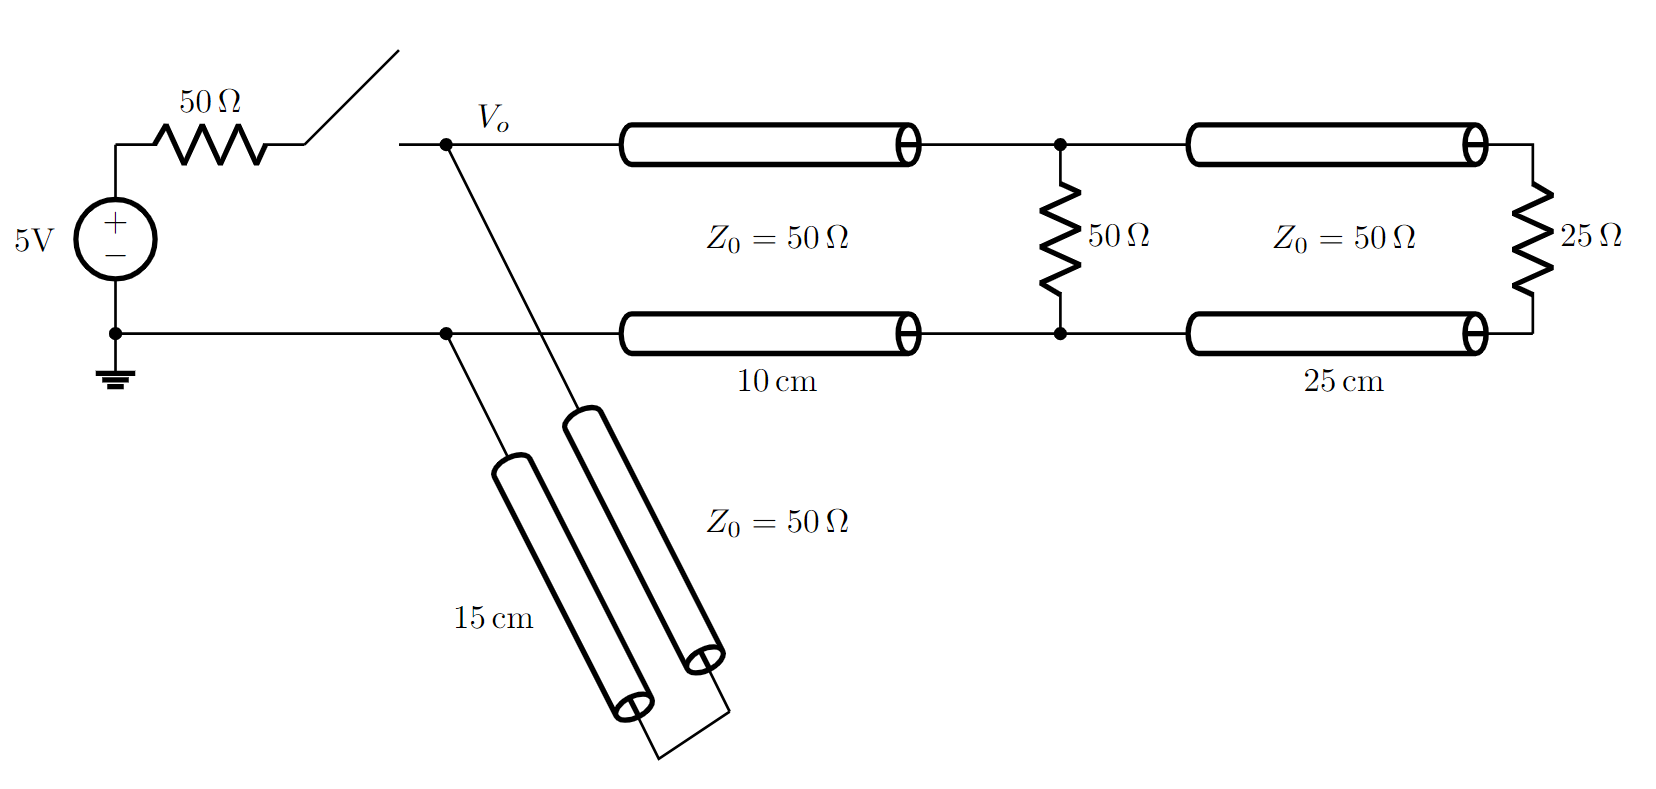
\includegraphics[width = 0.3\textwidth]{q2.png}
\end{center}
\end{figure}

\begin{enumerate}[label=(\alph*)]
    \item Donner l'évolution de de la tension $V_0$ à l'entrée du circuit pendant les 3.6 premières nanosecondes.
    \item  Donner la tension de sortie du générateur ($V_0$) en régime. Justifiez.
    \item  Après un temps suffisant pour que le circuit soit en régime, on coupe le générateur. Donner l'évolution de la tension $V_0$ à l'entrée du circuit pendant les 3.6 premières nanosecondes.
\end{enumerate}

\nosolution

\section{Question 3}

Un amplificateur présente une impédance d'entrée de 40-j30 $[\Omega]$. On désire l'adapter à une source dont l'impédance série est de 50 $[\Omega]$.
L'adaptation est réalisée en utilisant en cascade une ligne à \SI{75}{\ohm} et un adaptateur quart d'onde (d'impédance caractéristique au choix).

\begin{enumerate}[label=(\alph*)]
    \item Donnez la longueur de la ligne à 75 $[\Omega]$ (en longueurs d'onde de cette même ligne), ainsi que l'impédance caractéristique de la ligne au quart d'onde.
    \item Que peut-on faire pour adapter maintenant à 50+j20 $[\Omega]$ (au lieu de 50 $[\Omega]$) avec les mêmes types de lignes ?
\end{enumerate}


\nosolution

\section{Question 4}
On considère un repère cartésien XYZ. Une onde plane à polarisation circulaire gauche se propage dans le vide, dans la direction des X positifs. La longueur d'onde est dénotée par $\lambda$. Une boucle métallique carrée de côté $\lambda/4$ se situe dans le plan XY (les axes de symétrie de la boucle sont X et Y). La puissance par unité de surface est de 2 $[W/m^2]$


\begin{enumerate}[label=(\alph*)]
    \item Donnez une expression phasorielle du champ électrique de l'onde.
    \item À supposer que la boucle soit ouverte en un point donné, quelle est la tension qui apparaît aux bornes de cette boucle ouverte ?
    \item À supposer que l'on introduise maintenant une charge de R = 500 $[\Omega]$ dans cette section ouverte, quelle est la puissance dissipée dans cette charge ?
    \item Déduisez-en une aire effective comme le rapport entre cette puissance et la puissance par unité de surface de l'onde incidente. Tentez de donner votre réponse uniquement en fonction de la longueur d'onde, de l'impédance du vide et de la résistance R.
\end{enumerate}

N.B: Comme l'impédance R est grande, assez peu de courant circule dans la boucle et on négligera le champ rayonné par la boucle elle-même dans le calcul de la tension induite. On néglige aussi le champ directement diffracté par la boucle.

\nosolution

\end{document}
